%\pagestyle{fancy}
\chapter{ExperimentalSetup}
\label{ch:ExperimentalSetup}

\section{Sensors}
\subsection{IMU}
\begin{figure}[htb]
	\centering
	%todo Add 3d coordinate system and trim image
	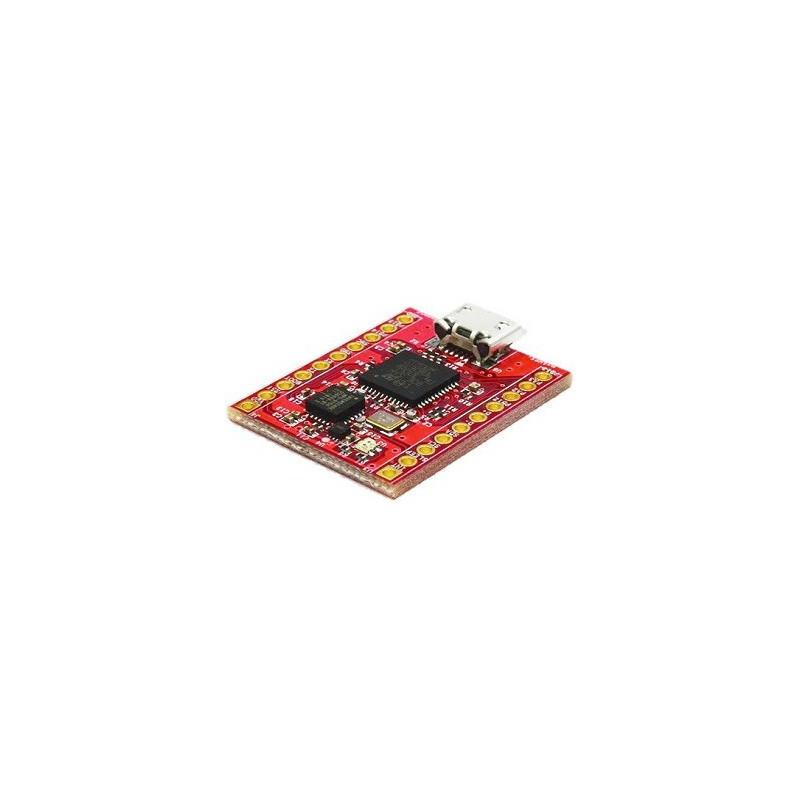
\includegraphics[clip, trim={8cm 8cm 8cm 8cm}, width=0.3\linewidth]{IMU.jpg}
	% 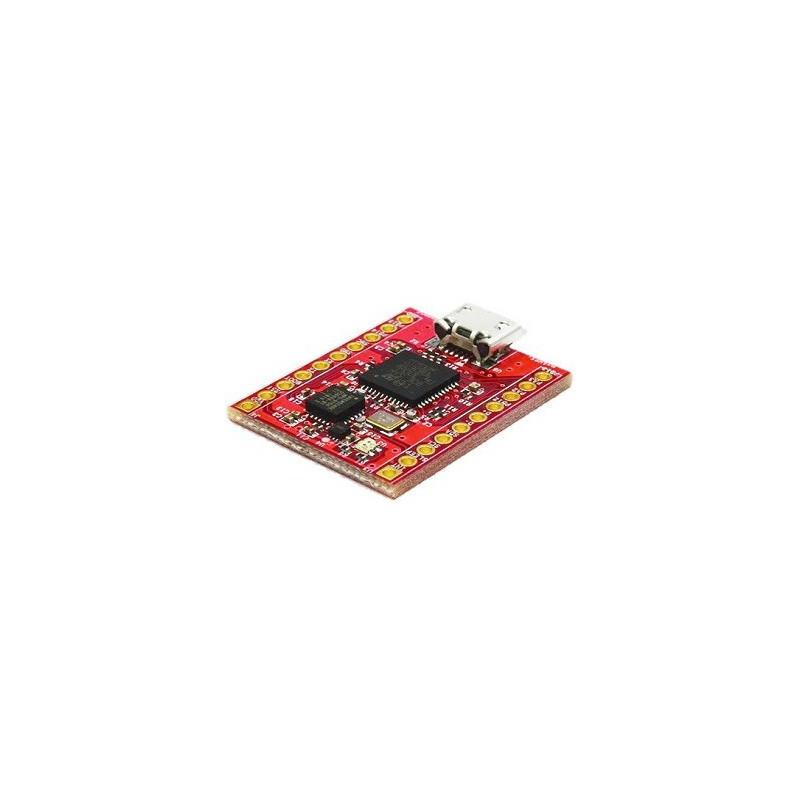
\includegraphics[width=0.7\linewidth]{IMU.jpg}
	\caption[myAIRS+ IMU]{myAIRS+ IMU this is the long caption which does not show up in list of figures \itodo{higher resolution + trim; add coordinate system}}
	\label{fig:imu}
\end{figure}
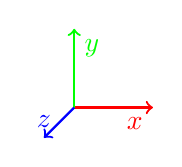
\begin{tikzpicture}
    \coordinate (O) at (0,0,0);
    \draw[thick,->, red] (0,0,0) -- (1,0,0) node[anchor=north east]{$x$};
    \draw[thick,->, green] (0,0,0) -- (0,1,0) node[anchor=north west]{$y$};
    \draw[thick,->, blue] (0,0,0) -- (0,0,1) node[anchor=south]{$z$};
\end{tikzpicture}

An \gls{imu} is used to track the orientation and position of an object. 
Common uses are in the aerospace or automotive industry, often in combination with other sensors, to give information about the pose and position of a vehicle. 
More recently with the invention of MEMS-IMUs \todo{might have to define MEMS here} which allow for a very small form factor at a low cost, IMUs are also used in consumer electronics such as smartphones or fitness tracker. 
An IMU usually consists of the three following sensors.
The acceleration is measured using an accelerometer and can be used to determine the velocity the covered distance by integrating once respectively twice.
The gyroscope gives information about the change of orientation. 
Often times a magnetometer is used as well, which is able to measure the earth's magnetic field and is used to correct the measurements of the gyroscope. It allows for the determination of the absolute heading, whereas the gyroscope can only measure relative change. But because it is very sensitive to other magnetic objects, it is often omitted.
IMUs can be typically divided into the two following categories.

In the first type, the stable platform systems, the inertial sensors are mounted such that they are always aligned with the reference frame.
This is achieved using gimbals, which allow movement along all three axes. 
The gyroscopes on the platform measure the rotation and send them to torque motors, which rotate the gimbals to keep the platform in alignment with the reference frame. 
The advantage of stable platform systems is that the calculation of orientation and position is straight forward. 
The angles of the gimbals can be measured to get the orientation and to get the position, the accelerometer measurements have to be be corrected for gravity (which is \SI{9.8}{\metre\per\second^2} in upward direction) and be integrated two times.
No coordinate transformation is necessary.
The disadvantages are that the mechanical structure of the setup is complex, needs regular maintenance, requires a lot of space and has high costs.

The second type are strapdown systems, which are mostly used today. \todo{reference?} 
As the name suggests all the parts are fixed onto the device and are thus not anymore always aligned with the reference frame.
Advantages are that due to the lack of gimbals and motors a significantly smaller build is possible and lower production costs can be achieved.
A disadvantage is that the calculation of the orientation and position is more complex, the rate gyroscopes have to be integrated to get the orientation and can then be used to transform the accelerometer signals into the reference frame.
But with the decrease of computational cost this disadvantages continues to diminish. And even though they are continually improved, the accuracy does not quite match the of strapdown systems.

There are many different types of gyroscopes and accelerometers such as mechanical, optical or solid state, but only the functionality of \gls{mems} will be described, because those will also be used in the experiment. Information about the working principle of other systems and also much more information about IMUs in general can be found in \cite{Woodman07anintroduction}.

MEMS consist of electrical and/or mechanical components in the size of \SI{100}{\nano\metre} to \SI{1}{\milli\metre}, allowing for a very small form factor.
Other characteristics of MEMS are that they can easily be mass produced allowing for low cost and usually also need less power than traditional systems, because everything is integrated on the chip \cite{Shaeffer2013}.
Almost all consumer grade electronics uses MEMS-IMUs nowadays, but they also find more and more use in non-critical industry segments \cite{Perlmutter2016}.

\subsubsection{MEMS Accelerometer}
\begin{figure}[htb]
	\centering
	%todo Better quality or create own fig
	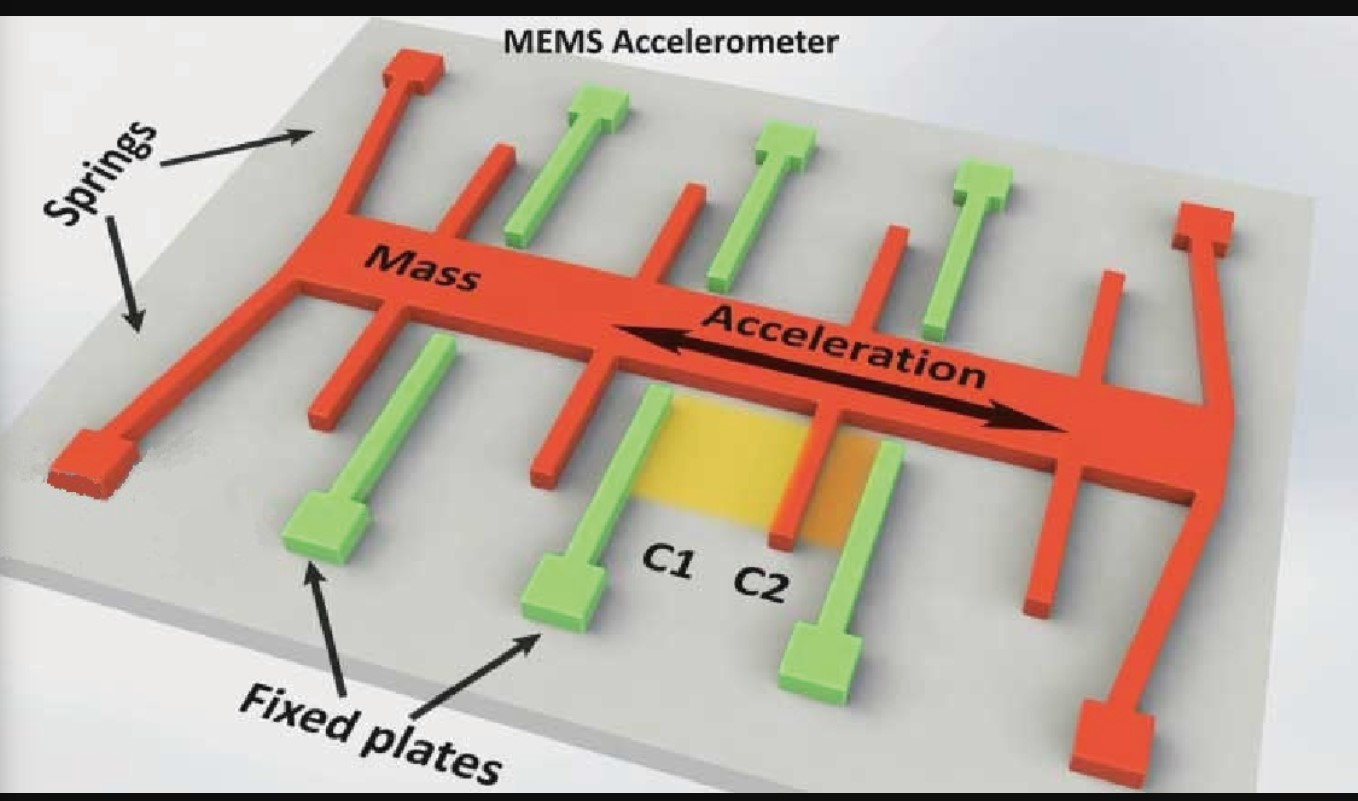
\includegraphics[width=0.7\linewidth]{MEMS_Accelerometer}
	\caption{Micro structure of a MEMS accelerometer }
	\label{fig:MEMS_Accelerometer}
\end{figure}
The accelerometer is used to measure the acceleration.
Besides dynamic acceleration there is the static and constant gravity acceleration on earth in upward direction. 
This allows for the determination of one axis of the IMU, even if it is not moving.
Often times only the dynamic acceleration are of interest, to get them the acceleration data during stand still must be measured and subtracted.
The micro structure of a MEMS accelerometer is shown in figure \ref{fig:MEMS_Accelerometer}.
A mass is suspended by springs along one axis and if an acceleration along this axis occurs, the mass moves in the opposite direction due to Newton's second law.
The mass has little fingers perpendicular to the moving direction axis, which affect the capacity between the fixed plates.
The change of capacity and thus voltage can be measured, from which the acceleration can be calculated.
To be able to measure the acceleration along all three axis the same setup is used three times, perpendicular to each other.

\subsubsection{MEMS Gyroscopes}
A gyroscope measures the angular velocity.
The setup of a MEMS gyroscope is similar to that of a MEMS accelerometer.
A proof mass is suspended on a frame and responds to an input force.
MEMS gyroscopes make use of the Coriolis effect, which states that an rotating object with the angular velocity $w$ of mass $m$ and velocity $v$ experiences a force
\[ F_C = -2m(w\times v). \]
To measure the effect, a mass is vibrating along one axis, which in turn is also suspended.
If the mass is oscillating along one axis and a rotation is applied, a second oscillation on the axis perpendicular to the rotation axis can be observed.
E.g.\ if the mass oscillates along the x-axis and a rotation around the z-axis is applied, a vibration along the y-axis can be observed.
By measuring the amplitude and phase of the secondary oscillation the absolute value and direction of the angular velocity can be calculated.
While MEMS gyroscopes do not achieve the same accuracy as optical gyroscopes they offer many advantages such as smaller physical properties (weight and size), lower power consumption and startup time as well as a significantly lower cost.
Optical gyroscopes cost in the range of \$10,000 whereas MEMS gyroscopes can cost as low as \$3 \cite{Perlmutter2016}.
But this comes at the cost of a worse angle drift which increases from 0.01 to 0.1 deg/h \todo{SIUnit} for optical gyroscopes to 10 deg/h \todo{check what type of deg/h there are, daytoday vs in-run} for MEMS-IMUs.
MEMS gyroscopes have replaced other gyroscope types in most areas, but in areas where the highest precision possible is necessary, typically in military industry, optical gyroscopes are still used today.

\subsubsection{(MEMS) Magnetometer}
\itodo{Sth sth lorenz (short because not used)}
The disadvantages are that the magnetometer is easily influenced by other ferromagnetic material and electronic devices.
Therefore indoor use while getting reliable data is rarely possible.

\subsubsection{Typical MEMS errors}
Maybe a sentence about idc about problems, because raw measurements are mostly used.
\todoin{
  \begin{itemize}
	\item Calibration errors
	\item Turn-On Bias
	\item Bias instability
	\item Bias Correction methods
	\item VERY BRIEF
  \end{itemize}}

\subsubsection{Used IMU}
For the experiments the myAHRS+, a low cost high performance \gls{ahrs} will be used.
An AHRS contains an IMU and outputs the raw data but also has an integrated Kalman filter which calculates the pose in form of quaternion or euler angles.
It offers an micro-USB interface and runs with up to \SI{100}{\Hz}.
It can capture a change of $\pm$2000 dps (degrees per second), $\pm$16 $g$ and $\pm$\SI{1200}{\micro\tesla}.
During the experiment only a fraction of this range is expected to be reached, hence the sensor seems suitable.
Besides the hardware the unit already has an Extended Kalman Filter (EKF) on board.
The EKF fuses the measurements of the three sensors and estimates a quaternion (and sth else?) from it.
But this will not be used.

\subsection{Lidar}
\begin{figure}[htb]
	\centering
	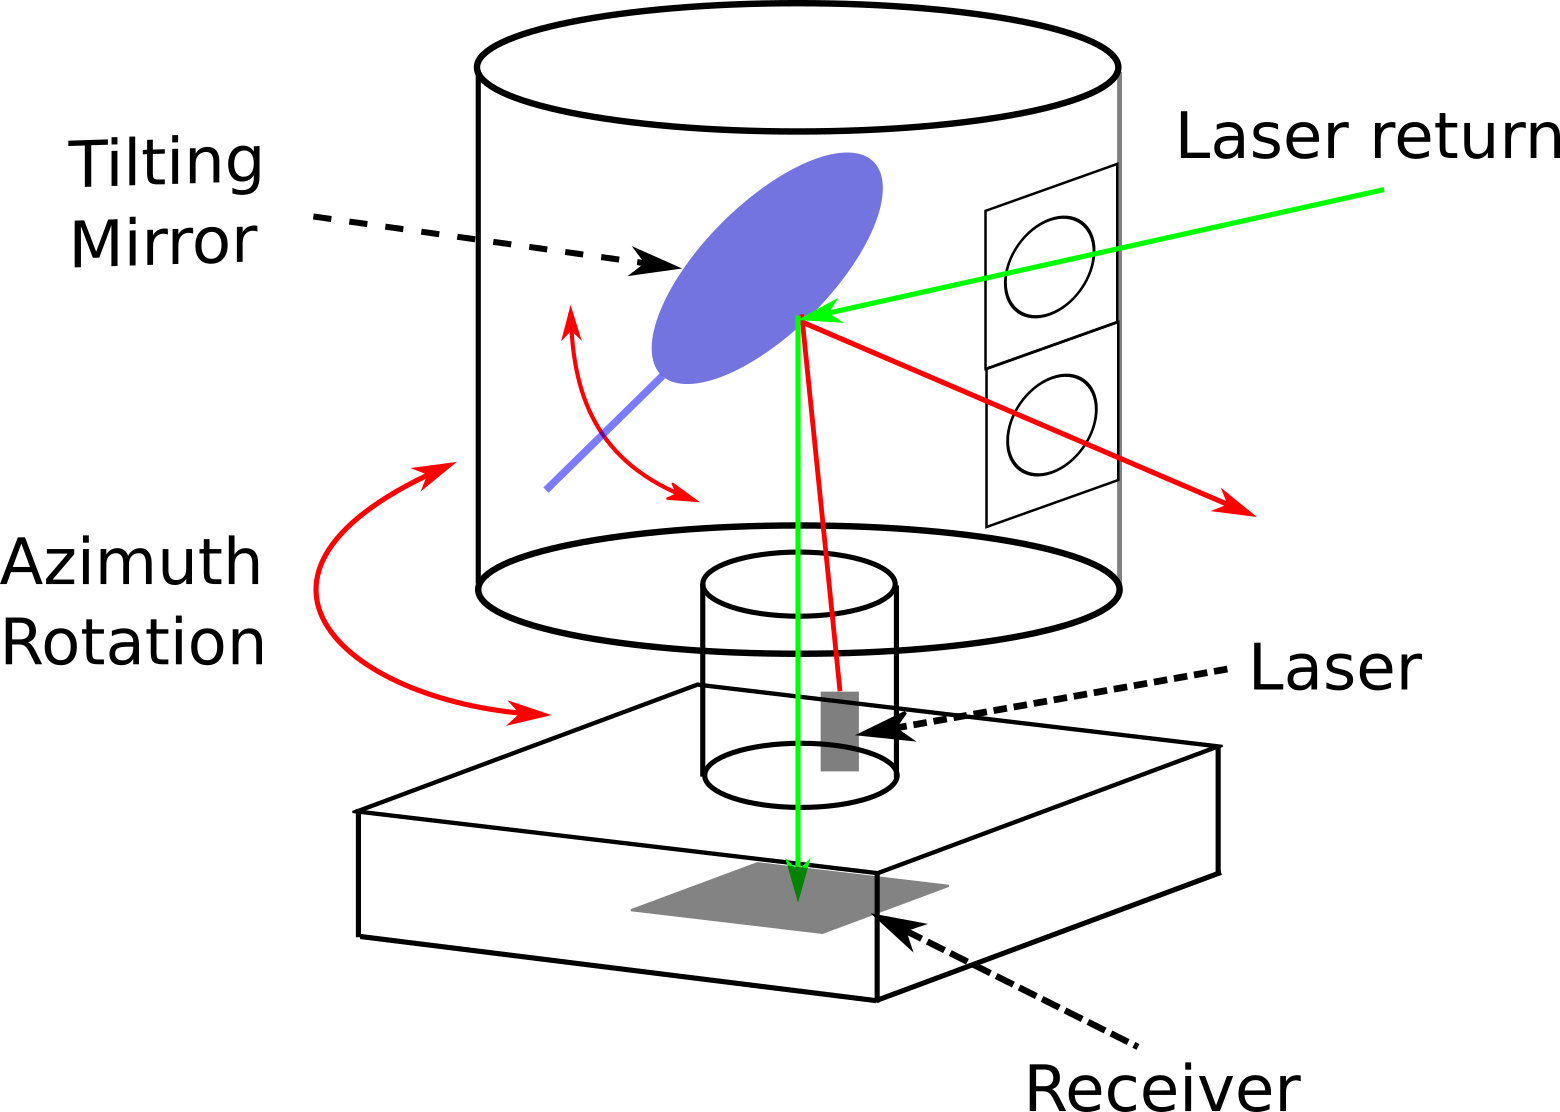
\includegraphics[width=0.5\textwidth]{Lidar.png}
	\caption{Setup of a mechanical spinning Lidar \cite{Li2020}}
	\label{fig:lidar}
\end{figure}
\textbf{LI}ght \textbf{D}etection \textbf{A}nd \textbf{R}anging or also known as \textbf{L}ight \textbf{I}maging, \textbf{D}etection \textbf{A}nd \textbf{R}anging (LIDAR) is a method to measure distance to objects.
Similar to other systems such as SONAR or RADAR, LIDAR uses the time-of-flight principle.
A short laser pulse is sent into the environment and the reflected light is analyzed.
The duration it took from sending to receiving gives information about the distance.
The intensity and wavelength of the returning light are measured as well and can provide information about the reflectivity of the object (intensity) or the chemical composition of the air (wavelength).
Common uses of LIDAR are the analysis of earth's atmosphere, 3D mapping of environments or in the field of autonomous driving for object detection, tracking and simultaneous localization and mapping (SLAM).
Basically all applications which use RADAR can also be used with a LIDAR instead, allowing for a greater accuracy.

There are different LIDAR types but the principles are similar.
A transmitter generates a signal and sends it into the environment using a scanning system and a transmission optic.
As transmitter a laser with a wavelength of \SIrange{850}{950}{\nano\metre} is typically used.
The scanning system allows the laser to explore a large area instead of only a single point by steering the light at different azimuths and vertical angles and can be divided in mechanical spinning or solid state systems.
Mechanical spinning systems is the oldest technology and is still mainly used today.
A mirror which can be rotated around an axis is used, allowing for a greater vertical field of view.
Also the whole LIDAR base on which the laser is mounted can be rotated independently from the mirror, allowing for a 360° horizontal view.
To get a sufficient resolution the mirror has to spin at very high speeds, but some LIDARs also use additionally a vertical array of lasers instead of only one to further increase the density of the generated point cloud.
While mechanical spinning systems are very precise, they are bulky, need a lot of power and are expensive.
The working principle of a LIDAR using the mechanical spinning method is shown in figure \ref{fig:lidar}.

Solid state systems and especially MEMS try to overcome those problems.
MEMS LIDAR are quasi-static, the only part that moves is the on the chip embedded mirror, but due to the small size (\SIrange{1}{7}{\milli\metre} diameter) very little power has to be used to move it.
They can be rotated on up to two axes, but because the laser cannot be rotated a horizontal view of 360° is not possible.
But advantages compared to mechanical systems are the smaller former factor and lower cost.

After transmitting the laser signal the reflected light passes through the receiving optic and is received by photodetectors.
A processing unit then generates a 3D point cloud from all the received measurements.

\itodo{Sort citations and maybe add some more}
\cite{Wang2020}
\cite{Vaughan2006}
\todoin{\begin{itemize}
		\item What is lidar and where used
		\item How does it work
		\item Advantages and disadvantages
		\item Information about lidar used in experiment
\end{itemize}}


\subsection{Used LiDAR}
Two different LiDARs will be used during the experiment.
The RS-Bpearl and the Velodyne UltraPuck.
The most relevant data can be seen in table \ref{tab:lidar_datasheets}.
Both are mechanical LiDARs and have the same number of laser channels, but the Velodyne has a significant better vertical resolution, due to the smaller vertical FOV.

\begin{table}[ht]
	\centering
	% todo: Manual citation prop wrong
	\caption{Comparison of the two used LiDARs \cite{RoboSense2020}\cite{Rev}}
	\label{tab:lidar_datasheets}
	\begin{tabular}[t]{lcc}
	\toprule
	&RS-Bpearl & Velodyne Ultra Puck\\
	\midrule
	Channels 				& 32 							& 32\\
	Range 					& \SI{100}{\metre}				& \SI{200}{\metre}\\
	Range accuracy			& $\pm\SI{3}{\centi\metre}$		& $\pm\SI{3}{\centi\metre}$\\
	Horizontal FOV		 	& \SI{360}{\degree}				& \SI{360}{\degree}\\
	Vertical FOV 			& \SI{90}{\degree}				& \SI{40}{\degree}\\
	Horizontal resolution	& \SIrange{0.2}{0.4}{\degree} 	& \SIrange{0.1}{0.4}{\degree}\\
	Vertical resolution		& \SI{2.81}{\degree} 			& \SI{0.33}{\degree}\\
	Frame rate 				& \SIrange{10}{20}{\hertz}		& \SIrange{5}{20}{\hertz}\\
	Laser wavelength 		& \SI{905}{\nano\metre} 		& \SI{903}{\nano\metre}\\
	% \midrule
	Points per second 		& 576,000						& 600,000		\\
	\bottomrule
	\end{tabular}
	\end{table}%

\missingfigure{Picture of robosense or/and velodyne}

\subsection{Odometry}
\todoin{
  \begin{itemize}
	\item What is it and where used
	\item very short how does it work
	\item maybe calculation of velocity from ticks here
  \end{itemize}}

\section{Car}
\missingfigure{Picture of eGolf}

\section{Garage}
\missingfigure{Picture of ramps or figure of ramps showing angles}


%\subsubsection{Mechanical}
%One of the earliest realization of a gyroscope and consists of a platform and three (or two?!) gimbals.  
%\subsection{Optical}
%More precise but also more expensive are optical gyroscopes. It uses the signac effect, which says that it takes longer to travel a circular path with the direction of rotation, than it does against. A coil of optical fiber with multiple loops is setup and a laser beam is sent in both directions and the interference of the two beams is measured. Due to the high speed of light the path has to be long enough (>\SI{100}{\metre}), to allow for a measurable result.